\documentclass[11pt]{article}
\usepackage[margin=1in]{geometry}
\usepackage{graphicx}
\usepackage{microtype}
\usepackage{verbatim}
\usepackage{amsmath}
\usepackage[colorlinks=false, pdfborder={0 0 0}]{hyperref}
\begin{document}
\title{Traffic Light Controller \& Jeopardy Game\\Embedded System Design, Lab 1}
\date{September 17, 2015}
\author{Ben Lorenzetti}
\maketitle
\tableofcontents

\section{Objectives and Problem Description}

The objectives of this lab were to learn the basics of the Stamp 2 board, setup the programming+debugging toolchain, and complete two projects with the simplest actuators available: LEDs and pushbutton switches.

\subsection{Traffic Light Controller}

The first project is the traffic light controller, which models two traffic lights at an intersection between a major and minor road. There are 6 LEDs--2 red, 2 yellow, 2 green--and a pushbutton switch representing a magnetic presence sensor on the minor road. The major road should always remain green unless the minor road pushbutton is triggered. This trigger causes a transistion following normal traffic signals, with 5 second delays between each signal permutation and 10 seconds green duration on the minor road.

\subsection{Jeopardy Style Game}

The second project has two pushbutton representing Jeopardy buzzers and some indicator LEDs.
When the go LED turns on, two players compete to buzz in the quickest.
The winner is displayed via LEDs and the winning player's reaction time is printed to the debug terminal.
To make the game more difficult and competitive, the go LED is delayed by a random amount of time.

\section{Procedure}

\subsection{Traffic Light Controller}

The lab said to go through the first 3 chapters of the book and do the activities, so I did this.

I built the circuit shown in \hyperref[traffic-light-circuit]{figure \ref{traffic-light-circuit}} on the Basic Stamp breadboard.
It has the 6 LEDs in active low configuration with $1k\Omega$ current limiting resistors.
The pushbutton switch was also configured active low for consistency.
It also has a $1k\Omega$ current limiting resistor.

\begin{figure}[h!]
\centering
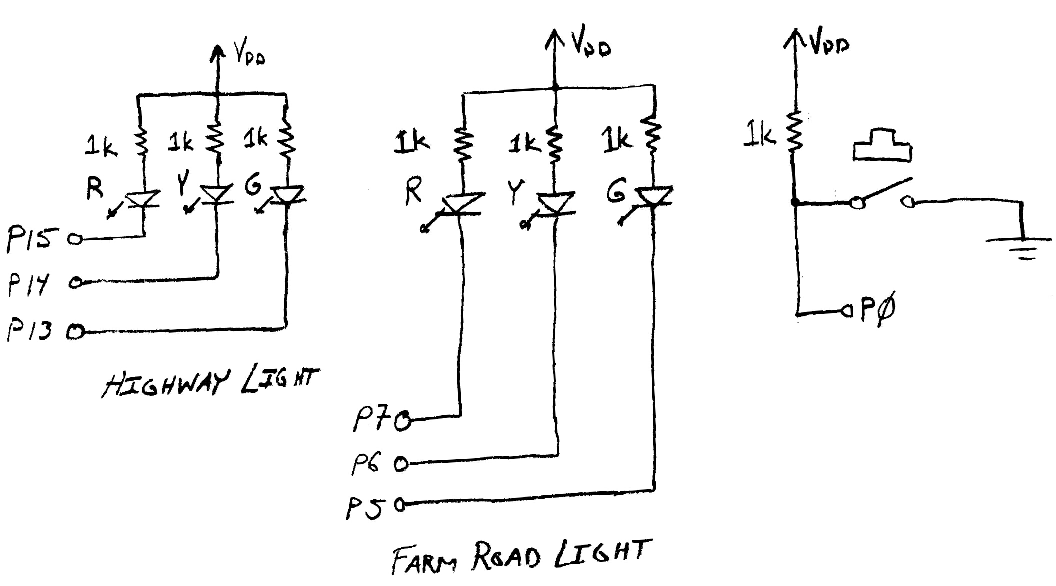
\includegraphics[width=.6\textwidth]{traffic-light-circuit.pdf}
\caption{Traffic Light Controller Circuit Diagram}
\label{traffic-light-circuit}
\end{figure}

The control flow chart for the PBasic program is shown in \hyperref[traffic-light-flowchart]{figure \ref{traffic-light-flowchart}}.

\begin{figure}[ht]
\centering
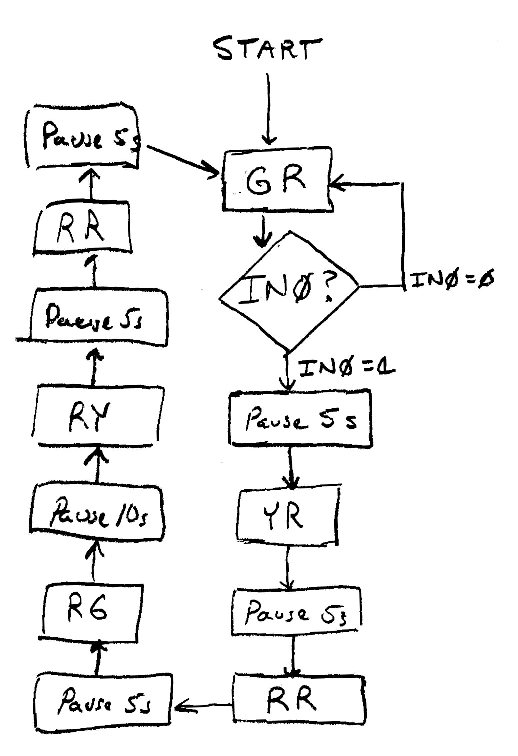
\includegraphics[width=0.3\textwidth]{traffic-light-flowchart.pdf}
\caption{Traffic Light Controller Flowchart}
\label{traffic-light-flowchart}
\end{figure}

\subsection{Jeopardy Style Game}

I designed the circuit for the Jeopardy game similarly to the traffic light controller.
Each LED or pushbutton switch has a $1k\Omega$ current limiting resistor and is configured active low.
The circuit diagram for the Jeopardy game is shown in \hyperref[jeopardy-circuit]{figure \ref{jeopardy-circuit}}.

\begin{figure}[h!]
\centering
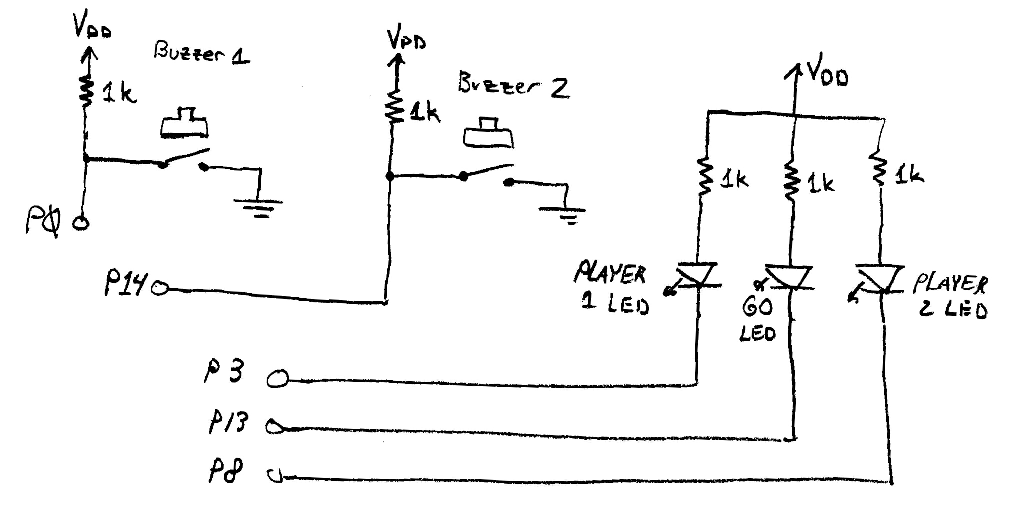
\includegraphics[width=0.7\textwidth]{jeopardy-circuit.pdf}
\caption{Jeopardy Circuit Diagram}
\label{jeopardy-circuit}
\end{figure}

The jeopardy game was more complicated than the traffic light controller,
but only from a software perspective--not hardware.

I used the random function to generate a random delay time before the game begins,
passing in the previous game's reaction time as a seed value so that the same
pseudorandom sequence is not repeated every game.

Once the game begins the microcontroller executes a tight loop that does checks the pushbuttons
for a victor and then increments a react\_cycles variable.
When the first player buzzes in, the appropriate LED lights up and their reaction
time is calculated from the number of cycles and the closest integer to the loop iteration time.
This value is printed to the debug terminal.

The control flow chart for the PBasic program is shown in \hyperref[jeopardy-flowchart]{figure \ref{jeopardy-flowchart}}.

\begin{figure}[ht]
\centering
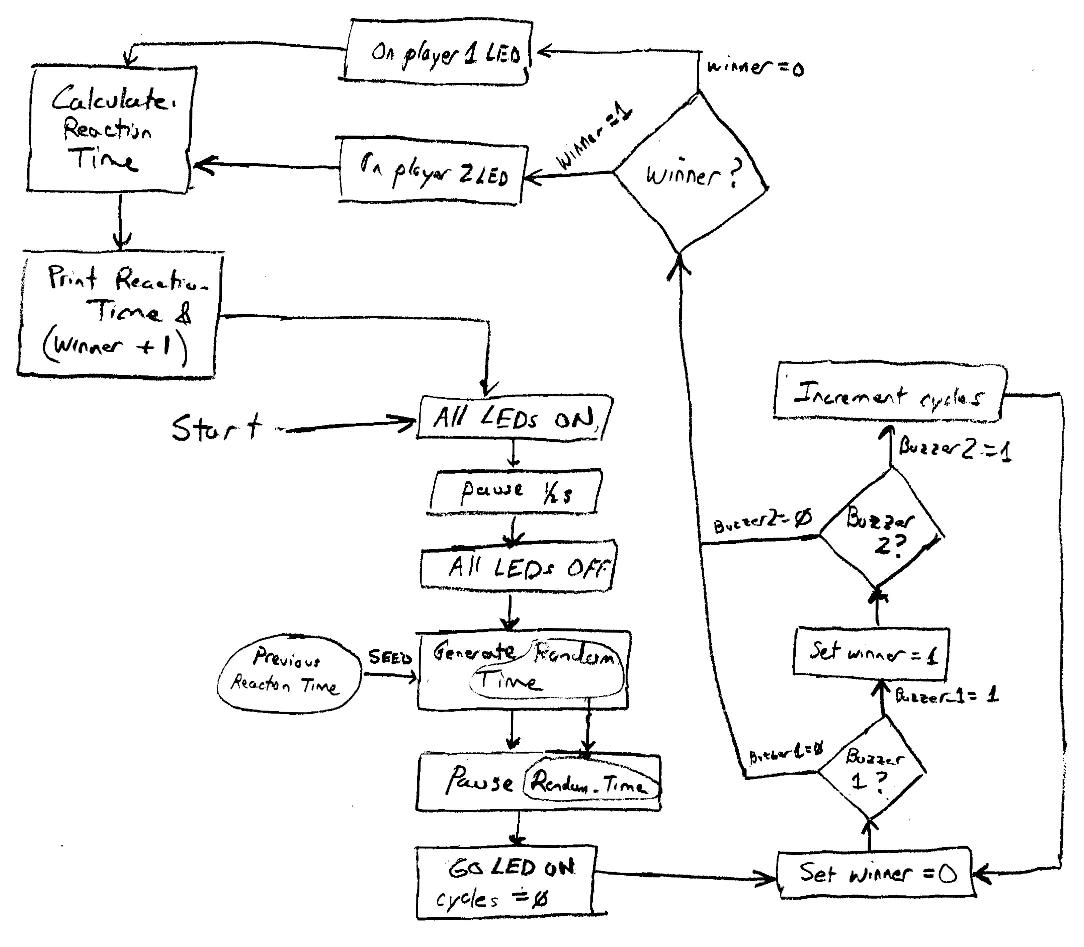
\includegraphics[width=0.7\textwidth]{jeopardy-flowchart.pdf}
\caption{Jeopardy-Like Game Flowchart}
\label{jeopardy-flowchart}
\end{figure}

\section{Expected Results}

I expected both circuits to behave according to the problem statements.

\section{Experiment and Design Revisions}

\subsection{Traffic Light Controller}

This circuit and code worked like a charm.
No revisions had to be made, but I did restyle the code to look more like C with boolean algebra.

\subsection{Jeopardy Game}

I really did not want to have two sets of Debug statements, depending on the winner.
However, using only one Debug statement and storing the winner in a bit variable proved more difficult than I anticipated.

It was difficult to generate the boolean algebra statements for turning on the appropriate LEDs,
mostly because PBasic sucks and doesn't even have a complete set of boolean operators.

So reducing to one set of Debut statements and only a single goto location proved more difficult,
but I think it was worth the change for code brevity.

\section{Observations}

Both circuits worked as expected, and photos of the working boards are shown in
\hyperref[traffic-light]{figure \ref{traffic-light}}
and \hyperref[jeopardy-board]{figure \ref{jeopardy-board}}.
A screenshot of the Debug terminal for the Jeopardy board is shown in figure \ref{jeopardy-screenshot}.

\begin{figure}
\centering
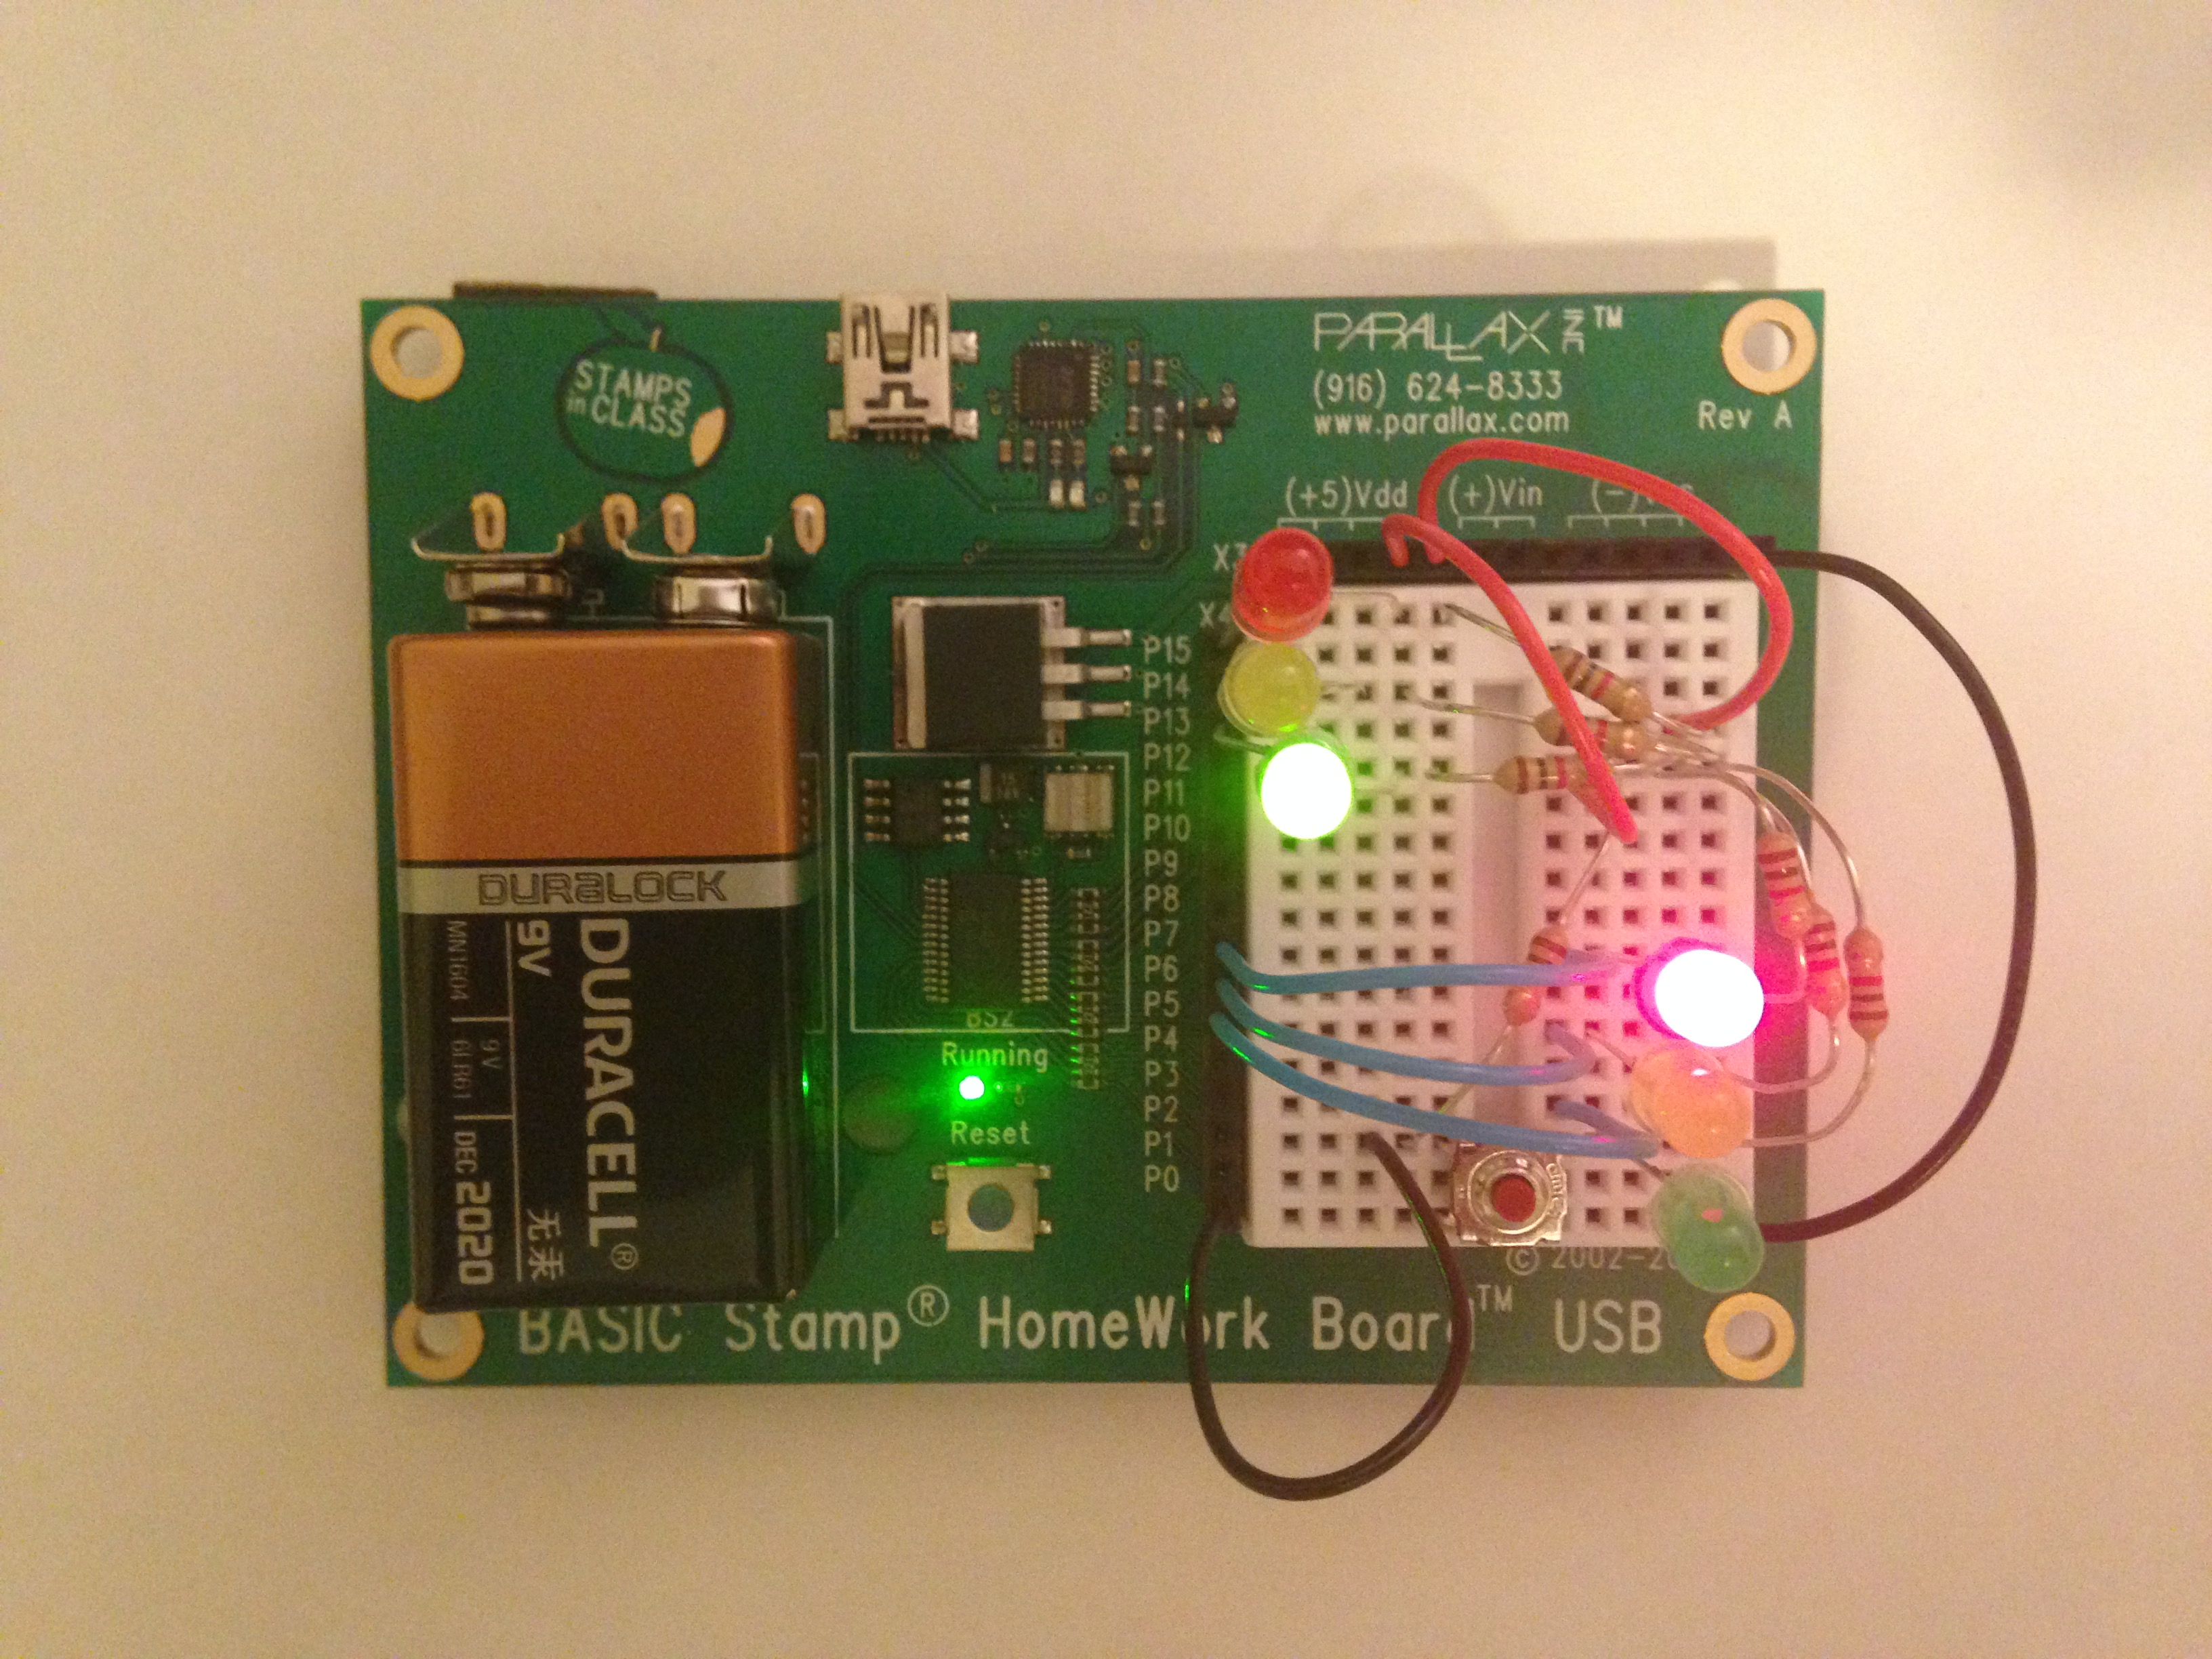
\includegraphics[width=0.6\textwidth]{traffic-light.jpg}
\caption{Traffic Light Controller Circuit}
\label{traffic-light}
\end{figure}

\begin{figure}
\centering
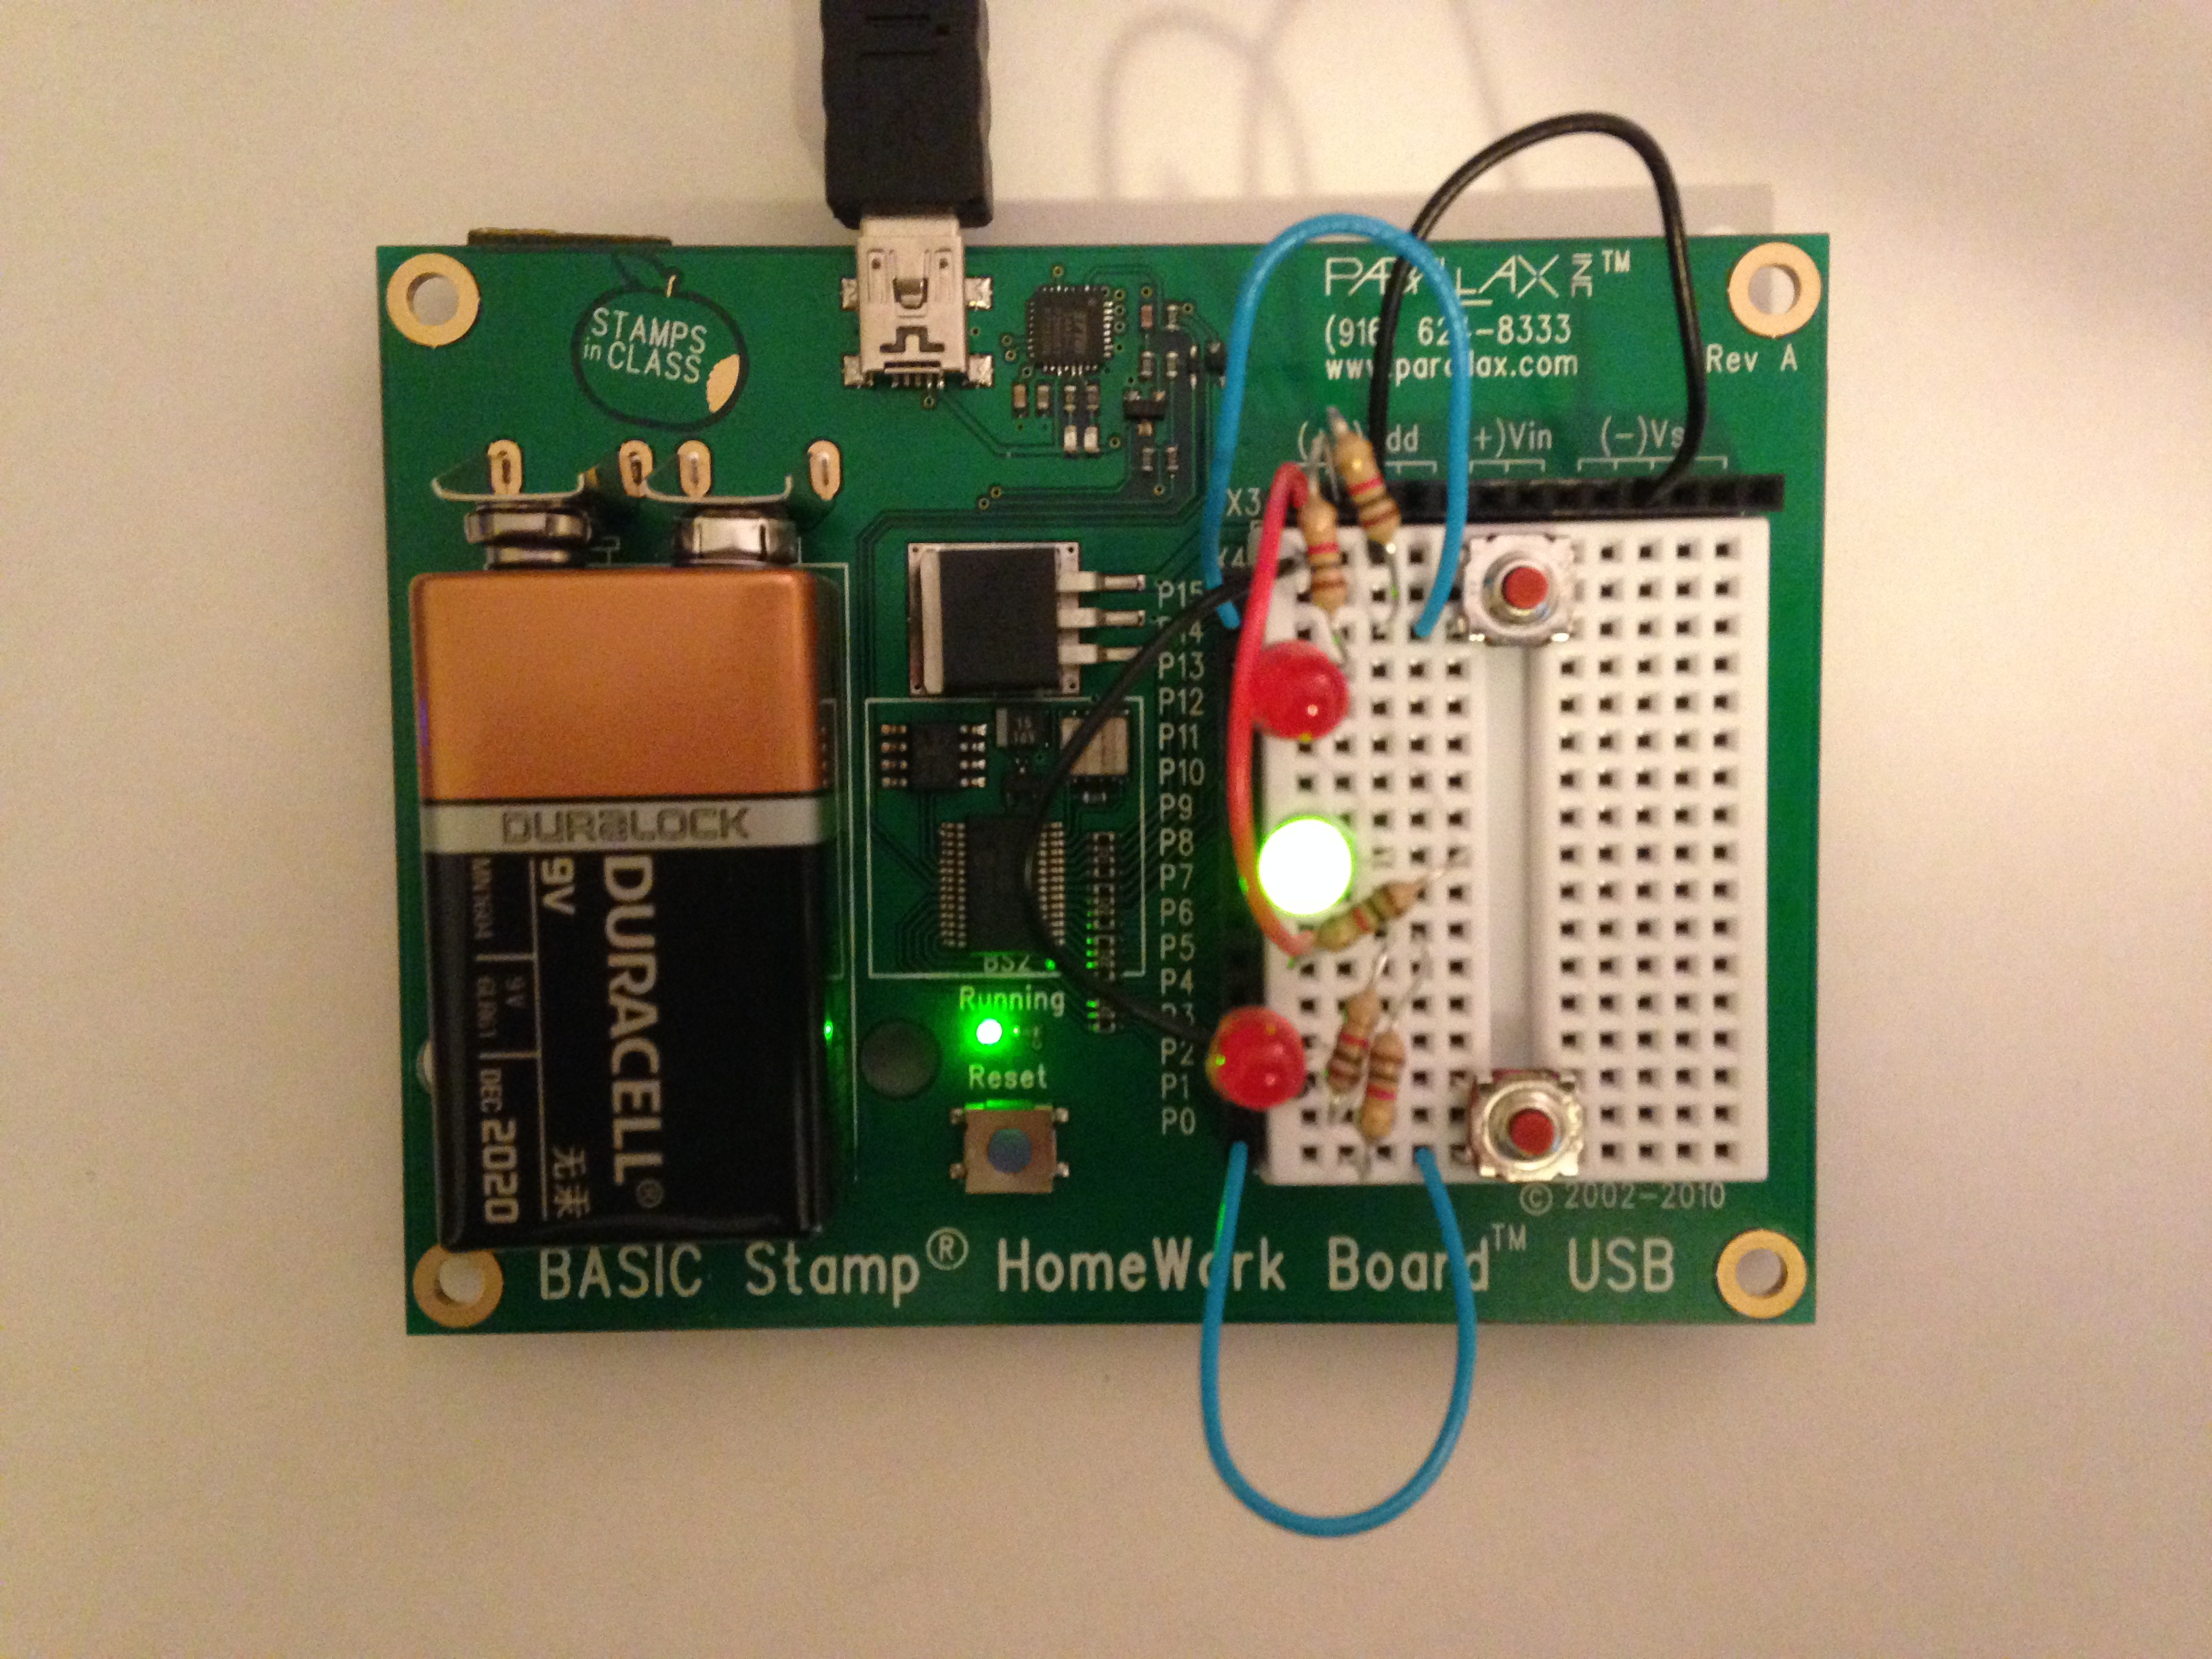
\includegraphics[width=0.6\textwidth]{jeopardy-board.jpg}
\caption{Jeopardy Game Circuit}
\label{jeopardy-board}
\end{figure}

\begin{figure}
\centering
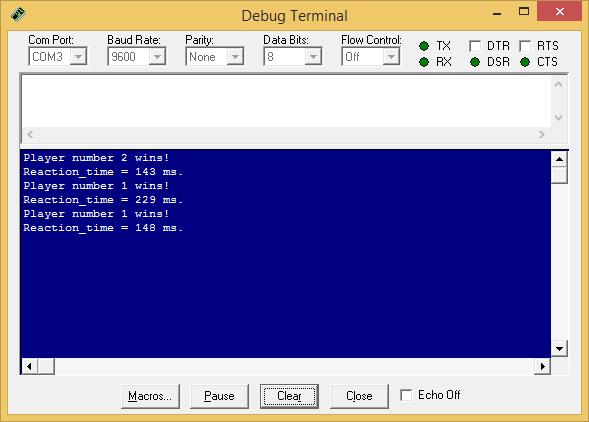
\includegraphics[width=0.75\textwidth]{jeopardy-screenshot.jpg}
\caption{Screenshot of Jeopardy Debug Terminal with Reaction Times}
\label{jeopardy-debug}
\end{figure}

\section{Discussion}

This lab really revealed a major flaw of the Stamp Basic board:
the fact that running an interpreter prevents you from knowing exact timing.
If we were writing code directly for PIC, we could no the clock rate and write some
assembly inside the reaction time loop--and therby no the exact number of clock cycles
and the clock rate.

I have a low opinion of the Stamp Basic board right now, at least compared to other
microcontrollers. This week I complain about not having control of clock cycles or there being
a clock variable that is accessable. Next weeks' dissatisfaction preview: no ADC on board.

\section{Exercises}

There were no exercises given.

\clearpage
\section{Programs}

\subsection{Traffic Light Controller}
\begingroup
\fontsize{10pt}{12pt}

\verbatiminput{Traffic-Controller.bs2}

\endgroup

\clearpage
\subsection{Jeopardy Style Game}
\begingroup
\fontsize{9pt}{11pt}

\verbatiminput{Jeopardy.bs2}

\endgroup

\end{document}
